\documentclass[a4paper,12pt]{article}
\usepackage{amsmath}
\usepackage{amsfonts}
\usepackage{amsthm}
\usepackage{amsfonts}
\usepackage{amssymb}
\usepackage{physics}
\usepackage{graphicx}
\usepackage{xcolor}
\begin{document}
\section*9
\[\begin{cases}
	\dv{y}{x}=f(x)\\
	(x,y)=(x_0,y_0)\\
\end{cases}\]
\subsection*{(i)}
Let the estimated value of \(y\) at \(x=x_1\) be \(y_1\).\\
By the Euler method,
\[\begin{aligned}
	y_1&=y_0+\Delta x\eval{\dv{y}{x}}_{x=x_0}\\
	&=\boxed{y_0+(x_1-x_0)f(x_0)}
\end{aligned}\]
By the improved Euler method,
\[\begin{aligned}
	y_1&=y_0+\Delta x\frac{\eval{\dv{y}{x}}_{x=x_0}+\eval{\dv{y}{x}}_{x=x_1}}{2}\\
	&=\boxed{y_0+(x_1-x_0)\frac{f(x_0)+f(x_1)}2}
\end{aligned}\]
\subsection*{(ii)}
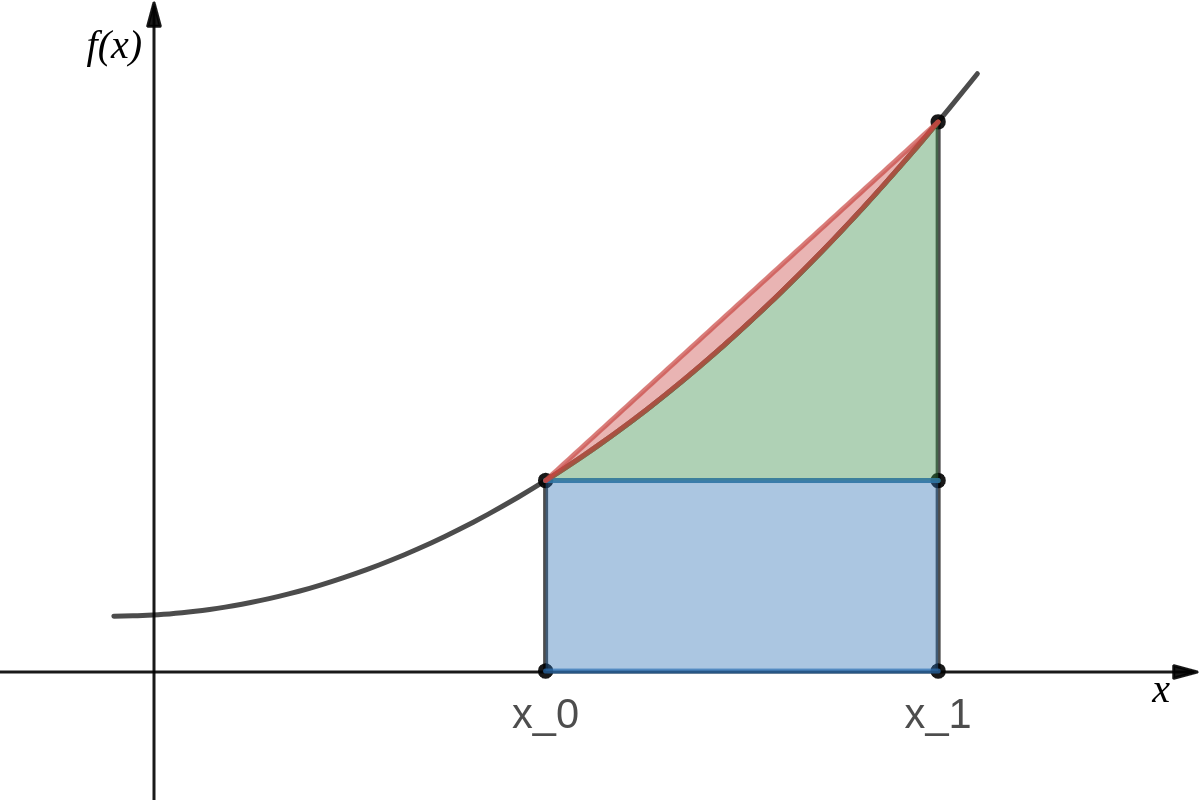
\includegraphics[width=\textwidth]{euler.png}
For the Euler method,
\[\begin{aligned}
    \Delta y&=y(1)-y_1\\
            &=\pqty{y_0+\int_0^1f(x)\dd{x}}-\pqty{y_0+(x_1-x_0)f(x_0)}\\
            &=\textcolor{green}B+\textcolor{blue}C-\textcolor{blue}C\\
            &=\textcolor{green}B\\
            &>0
\end{aligned}\]
For the improved Euler method,
\[\begin{aligned}
    \Delta y&=y(1)-y_1\\
            &=\pqty{y_0+\int_0^1f(x)\dd{x}}-\pqty{y_0+(x_1-x_0)\frac{f(x_0)+f(x_1)}2}\\
            &=\textcolor{green}B+\textcolor{blue}C-\textcolor{red}A-\textcolor{green}B-\textcolor{blue}C\\
            &=-\textcolor{red}A\\
            &<0
\end{aligned}\]
\subsection*{(iii)}
\[\begin{aligned}
	\dv{y}{x}&=a+bx+cx^2\\
	y&=d+ax+\frac b2x^2+\frac c3x^3
\end{aligned}\]
\[\begin{aligned}
	y_0&=d+ax_0+\frac b2x_0^2+\frac c3x_0^3\\
    y_0&=d+a{(0)}+\frac b2{(0)}^2+\frac c3{(0)}^3\\
	d&=y_0
\end{aligned}\]
\[\begin{aligned}
	y&=y_0+ax+\frac b2x^2+\frac c3x^3\\
	y(h)&=y_0+ah+\frac b2h^2+\frac c3h^3\\
	&=y_0+\frac h6\pqty{6a+3bh+2ch^2}
\end{aligned}\]
\[\begin{aligned}
	y_1&=y_0+(x_1-x_0)\frac{f(x_0)+f(x_1)}2\\
	y_1&=y_0+(h-0)\frac{f(0)+f(h)}2\\
	&=y_0+h\frac{a+a+bh+ch^2}2\\
	&=y_0+\frac h6\pqty{6a+3bh+3ch^2}
\end{aligned}\]
\[\begin{aligned}
	\Delta y&=y(h)-y_1\\
	&=\pqty{y_0+\frac h6\pqty{6a+3bh+2ch^2}}-\pqty{y_0+\frac h6\pqty{6a+3bh+3ch^2}}\\
	&=y_0+\frac h6\pqty{6a+3bh+2ch^2}-y_0-\frac h6\pqty{6a+3bh+3ch^2}\\
	&=\frac h6\pqty{6a+3bh+2ch^2-6a-3bh-3ch^2}\\
	&=\frac h6\pqty{-ch^2}\\
	&=\boxed{-\frac{ch^3}6}
\end{aligned}\]
\end{document}
